\chapter{Síntesis de imágenes de radiointerferometría}
\label{cap:imagesynthesisinterferometry}

\section{Atacama Large Millimeter-Submillimeter Array}

El Atacama Large Millimeter-Submillimeter Array (ALMA) es un radiointerferómetro compuesto de 66 antenas de alta precisión que operan a un ancho rango de frecuencias milimétricas y submilimétricas. Cincuenta de estas antenas miden 12 metros de diámetro y son utilizadas para síntesis de imágenes de alta resolución. Por otra parte, esto es complementado por el \textit{Atacama Compact Array} también llamado \textit{Morita Array} compuesto por doce antenas de 7 metros de diámetro y por otras 4 antenas de 12 metros diámetro para observaciones de poder total (\textit{Total Power}).

El conjunto de antenas está ubicado en el llano Chajnantor a 5.000 metros sobre el nivel del mar, un sitio que ofrece un cielo claro y un aire seco, una condición ambiental requerida para observar ondas milimétricas y submilimétricas.

La distribución de las antenas cede paso a lo que es llamado \textit{baseline} o distancia entre un par de antenas, que van desde 15 Km. hasta 16 Km. aproximadamente. Tanto la distribución de antes como la distancia entre éstas es crucial en la determinación de la calidad de la imagen y la resolución de ALMA.

\begin{figure}[h!]
\centering
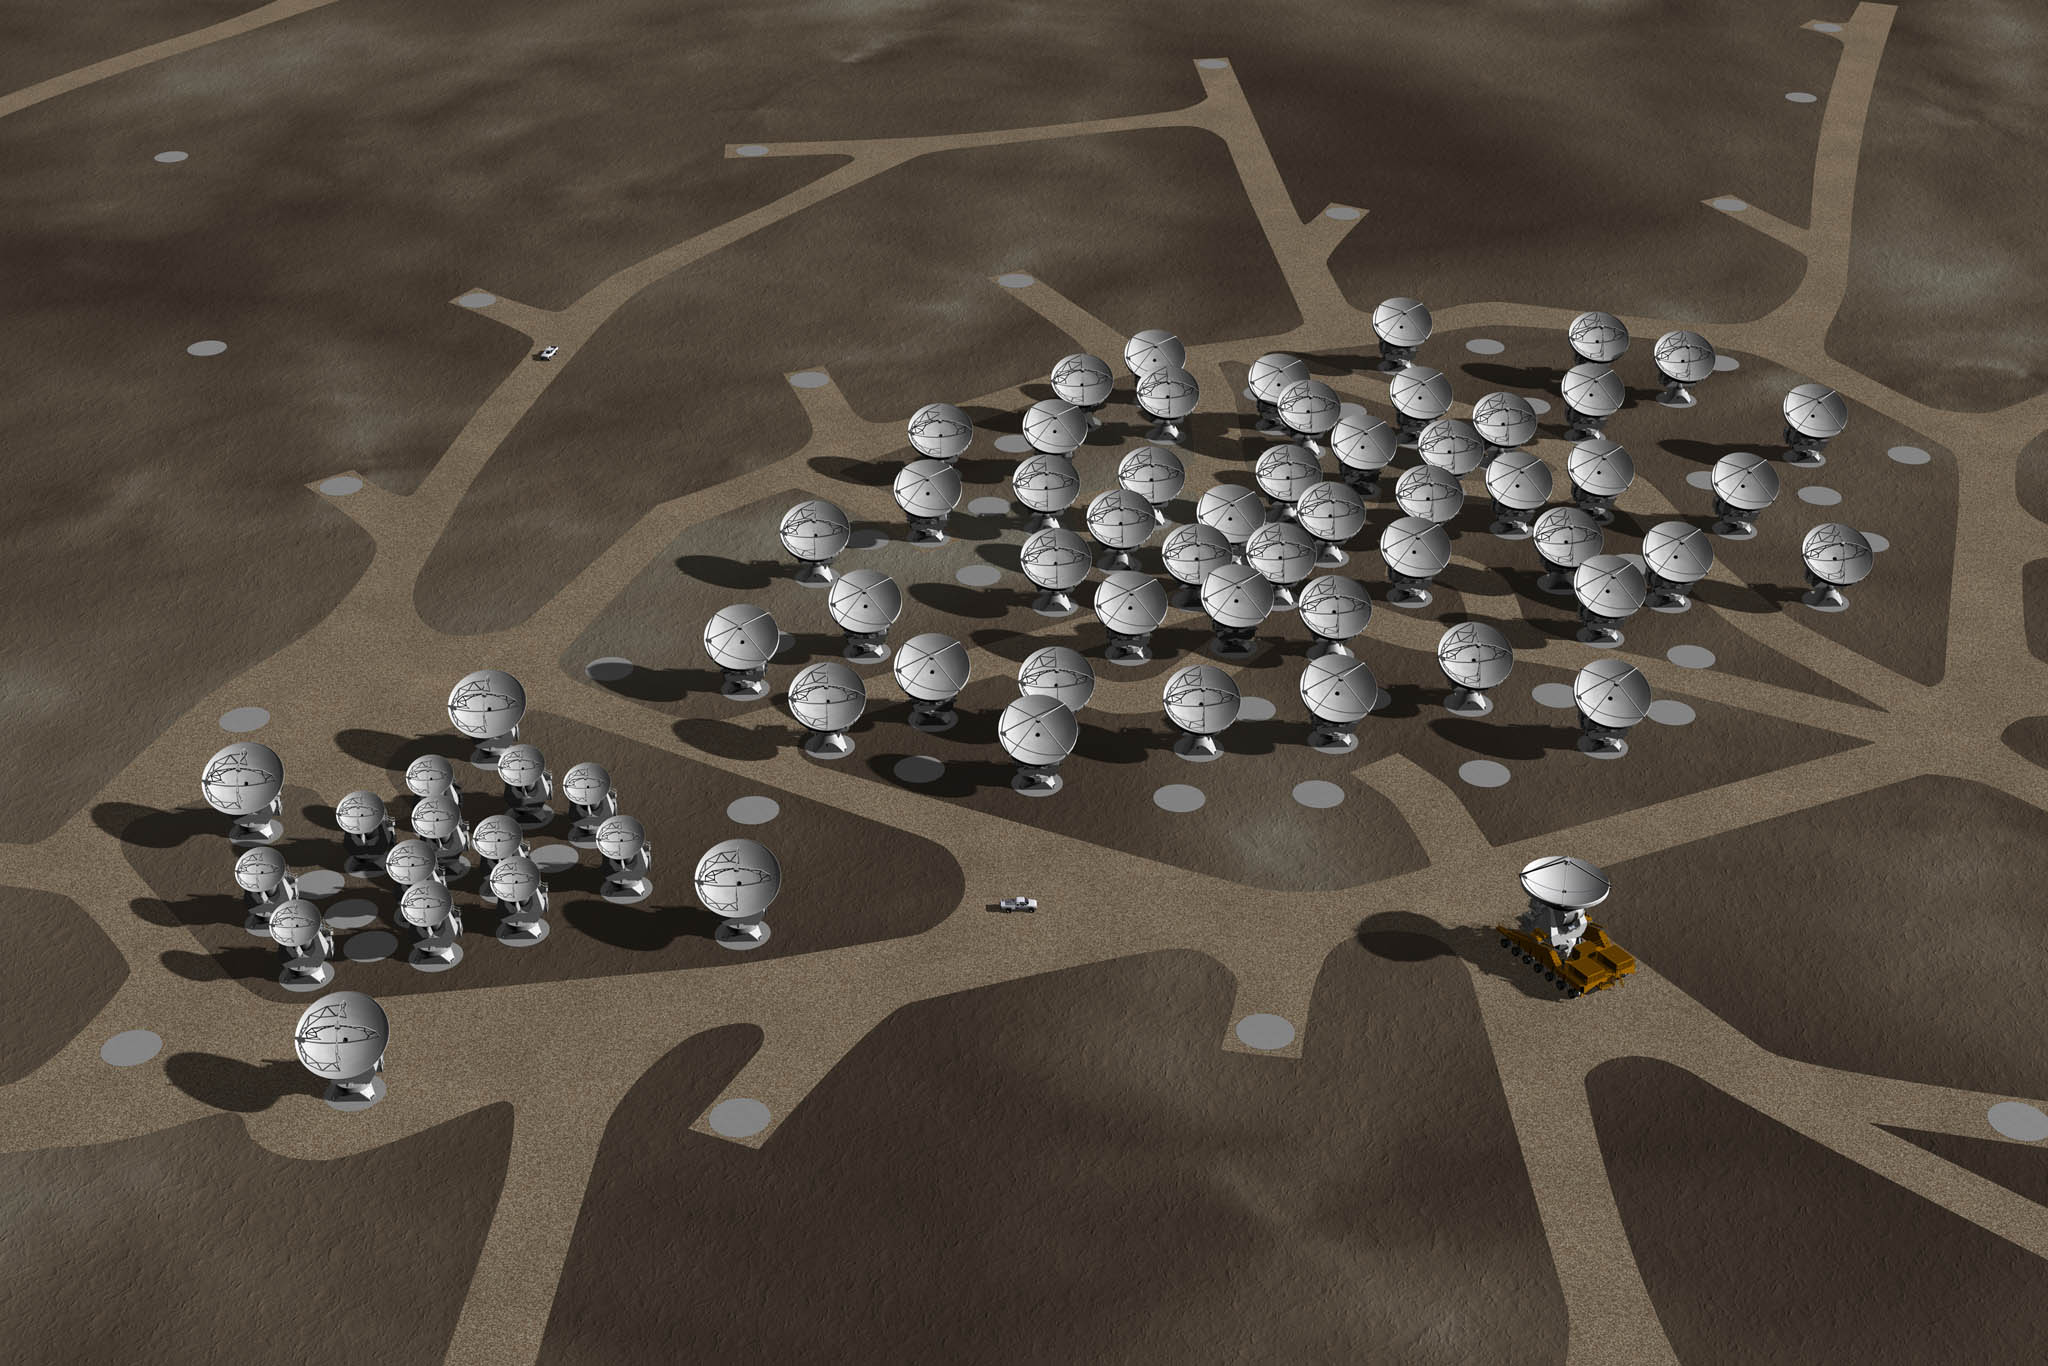
\includegraphics[scale=0.1]{images/almaarray.jpg}
\caption{Distribución de antenas en el llano Chajnantor. Fuente: ALMA (ESO/NAOJ/NRAO)}
\label{fig:almaarray}
\end{figure}


\clearpage

Por otro lado, cada antena contiene un receptor (también llamado \textit{Front-end}) que permite que las éstas capten información en diez bandas de frecuencia diferentes. Para ello cada antena está equipada con un criostato y su criorefrigerador adjunto. Estos criostatos contienen receptores que están montados y pueden ser reemplazados de forma fácil. En la tabla \ref{tab:bands} se adjuntan los datos de las distintas bandas de frecuencia que ALMA puede cubrir gracias a su front-end.

\newcommand{\ra}[1]{\renewcommand{\arraystretch}{#1}}
\begin{table}[h!]
\centering
\ra{1.2}
\caption{Las 10 Bandas de frecuencia de ALMA}
\label{tab:bands}
\begin{tabular}{@{}rcrrcr@{}} 
\toprule
 \multicolumn{1}{c}{{\bf Banda}} & \phantom{a} & \multicolumn{2}{c}{{\bf Rango de frecuencia (GHz)}}  & \multicolumn{1}{c}{{\bf Temperatura (K)}} \\
 \midrule
 1   && 31 - 45 &&  26\\
 2   && 67 - 90 &&  47\\    
 3  && 84 - 116 &&  60\\
 4  && 125 - 163 &&  82\\
 5  && 162 - 211 &&  105\\
 6  && 211 - 275 &&  136\\
 7  && 275 - 373 &&  219\\
 8  && 385 - 500 &&  292\\
 9  && 602 - 720 &&  261\\
 10  && 787 - 950 &&  344\\
 \toprule
\end{tabular}
\end{table}

Luego de que las ondas milimétricas y submilímetricas son recibidas por las antenas, éstas deben ser discretizadas y llevadas al correlacionador. El correlacionador recibe señales de voltaje desde cada antena, calcula la correlación cruzada y autocorrelación para éstas por cada par de antenas (\textit{baselines}), y produce las visibilidades complejas que los astrónomos reciben para sintetizar imágenes \citep{alma-handbook}. Para entender de mejor forma qué son las visibilidades es necesario conocer los conceptos esenciales de interferometría.

\section{Principios y conceptos de interferometría}

La interferometría es una técnica usada para obtener imágenes de alta resolución angular de un fenómeno astronómico particular. Esta implica la combinación de señales recibidas desde el cielo por dos antenas separadas físicamente. Estas señales contienen ruido, permitiendo así que la distribución del brillo del cielo sea muestreada en una escala angular más pequeña que la de una sola antena. 

La resolución angular de un interferómetro, $\delta$, es el angulo más pequeño en el que dos objetos pueden ser separados en orden de distinguirlos como objetos diferentes. Usando la teoría de la difracción, se puede demostrar que que para un interferómetro circular en particular de diámetro $D$, y una radiación de longitud de onda $\lambda$, este valor es $\delta \propto \frac{\lambda}{D}$. Esto quiere decir, que para grandes longitudes de onda (pequeñas frecuencias), se necesita un gran telescopio para obtener una buena resolución. Sin embargo, existen límites prácticos para construir un telescopio de un gran tamaño. Es por ello que haciendo uso de un conjunto de interferómetros situados a una distancia $D$, es posible obtener la misma resolución que una solo telescopio de radio $D$.



La relación entre la distribución del brillo del cielo y una visibilidad compleja está dada por el teorema de van Cittert-Zernike y es la base de la interferometría. Dado que los interferómetros no obtienen la imagen del cielo directamente, sino que obtienen visibilidades, que son que son la transformada de Fourier de la distribución del brillo del cielo en el plano de la imagen. Es decir, cada par de antenas forma un vector $\vec{k} = (u,v)$ en el plano de Fourier. Así mismo, la distribución del brillo del cielo es la transformada inversa de Fourier de las visibilidades complejas. Por lo tanto, la visibilidad $V(\vec{k})$ para un par de antenas con un \textit{baseline} $\vec{k}$, y su respectiva transformada inversa es:

%\begin{equation}
%V(\vec{k}) = \int_{-\infty}^{+\infty} A(\vec{x})I(\vec{x})e^{2\pi i %\vec{k}\vec{x}}\frac{dx dy}{\sqrt{1-x^{2}-y^{2}}}
%\end{equation}

\begin{align}
V(\vec{k}) &= \int\int A(\vec{x})I(\vec{x})e^{-2\pi i\vec{k}\vec{x}}dxdy \\
A(\vec{x})I(\vec{x}) &= \int\int V(\vec{k})e^{2\pi i\vec{k}\vec{x}}dudv
\end{align}

Donde $\vec{x} = (x,y)$ son las coordenadas del objeto a observar y estudiar, $A(\vec{x})$ es el \textit{primary beam}, $I(\vec{x})$ es la intensidad del objeto en $\vec{x}$, y $\vec{k}$ es el vector que se forma por cada par de antenas. 

\begin{figure}[h!]
\centering
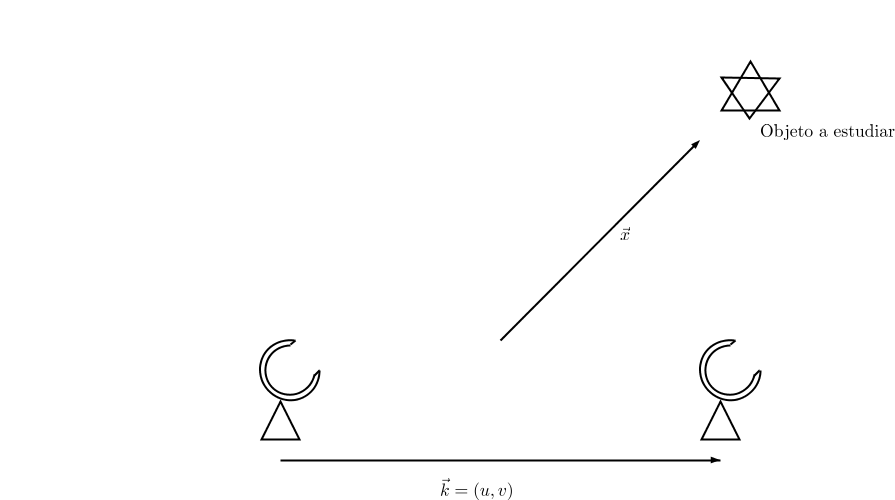
\includegraphics[scale=0.4]{images/antenas.png}
\caption{Dos antenas y su respectivo \textit{baseline}. $\vec{x}$ es la posición del objeto estudiado, y por otro lado $\vec{k}$ es el \textit{baseline} correspondiente a las dos antenas.}
\label{fig:antena}
\end{figure}

Esto quiere decir que la imagen de la distribución del brillo del cielo puede recuperarse a través del muestreo de la distribución de visibilidades complejas en el plano $(u,v)$. En esencia, una imagen es la transformada de Fourier de las visibilidades donde cada una de éstas tiene una amplitud y una fase representando el brillo y la posición relativa de la emisión en una escala angular específica.

%Debido a que existe un número finito de pares de antenas, al llevar a cabo una transformada de Fourier inversa aparecen \textit{side-lobes} rodeando al \textit{primary beam}. Los \textit{side-lobes} son irregularidades en los patrones de radiación debido a la extensión finita de los puntos en el plano $(u,v)$ y a deficiencias en la cobertura. La transformada inversa de Fourier aplicada a las visibilidades es llamada \textit{dirty map}. El \textit{dirty map} ($I_{D}$) es la imagen del cielo ($I_{sky}$) convolucionada con el \textit{beam} del interferómetro ($B$).

%\begin{equation}
%I_{D} = I_{sky} \ast B
%\end{equation}  

%El \textit{beam} $B$ para un interferómetro con un conjunto de \textit{baselines} $\{\vec{k}_{k}\}$ puede ser representado por la transformada inversa de Fourier de una suma de diferencias en estos puntos en el plano $(u,v)$. 

%\begin{align}
%B(\vec{x}) &= \int_{-\infty}^{+\infty}\sum_{k}\delta(\vec{k}-\vec{k}_{k})e^{2 \pi i \vec{k}_{k}\vec{x}}dudv \\
%&= \sum_{k}\left(\cos(-2\pi\vec{k}_{k}\vec{x})+i\sin(-2\pi\vec{k}_{k}\vec{x})\right) \\
%&= \sum_{k}\cos(2\pi\vec{k}_{k}\vec{x})
%\end{align}

Los datos astronómicos resultan desde la adición de el ruido instrumental hasta la convolución de la imagen del cielo con la respuesta instrumental. Debido al muestro incompleto en el plano $(u,v)$, la obtención de una imagen del cielo se convierte en un problema inverso que requiere algoritmos de síntesis de imágenes. 


\section{Métodos existentes de deconvolución} 



 
 










\chapter{GPGPU}
\label{cap:gpgpu}

\section{Arquitectura Unificada de Dispositivos de Cómputo}
\subsection{Arquitectura}
\subsection{Peer-to-Peer}
\subsection{Direccionamiento virtual unificado}
\subsection{GPUVMEM}

\chapter{Pruebas}
\label{cap:pruebas}

\chapter{Resultados}
\label{cap:resultados}